\documentclass{article}

\usepackage{graphicx}
\usepackage{tikz}
\usepackage{tikzsymbols}
\usetikzlibrary{calc,patterns,shapes.geometric}
\pagestyle{empty}
\usepackage[margin=0pt]{geometry}
\geometry{papersize={14in,12in}}

\def\centerarc[#1](#2)(#3:#4:#5){\draw[#1] ($(#2)+({#5*cos(#3)},{#5*sin(#3)})$) arc (#3:#4:#5);}

\begin{document}
	\begin{figure}
		\centering
		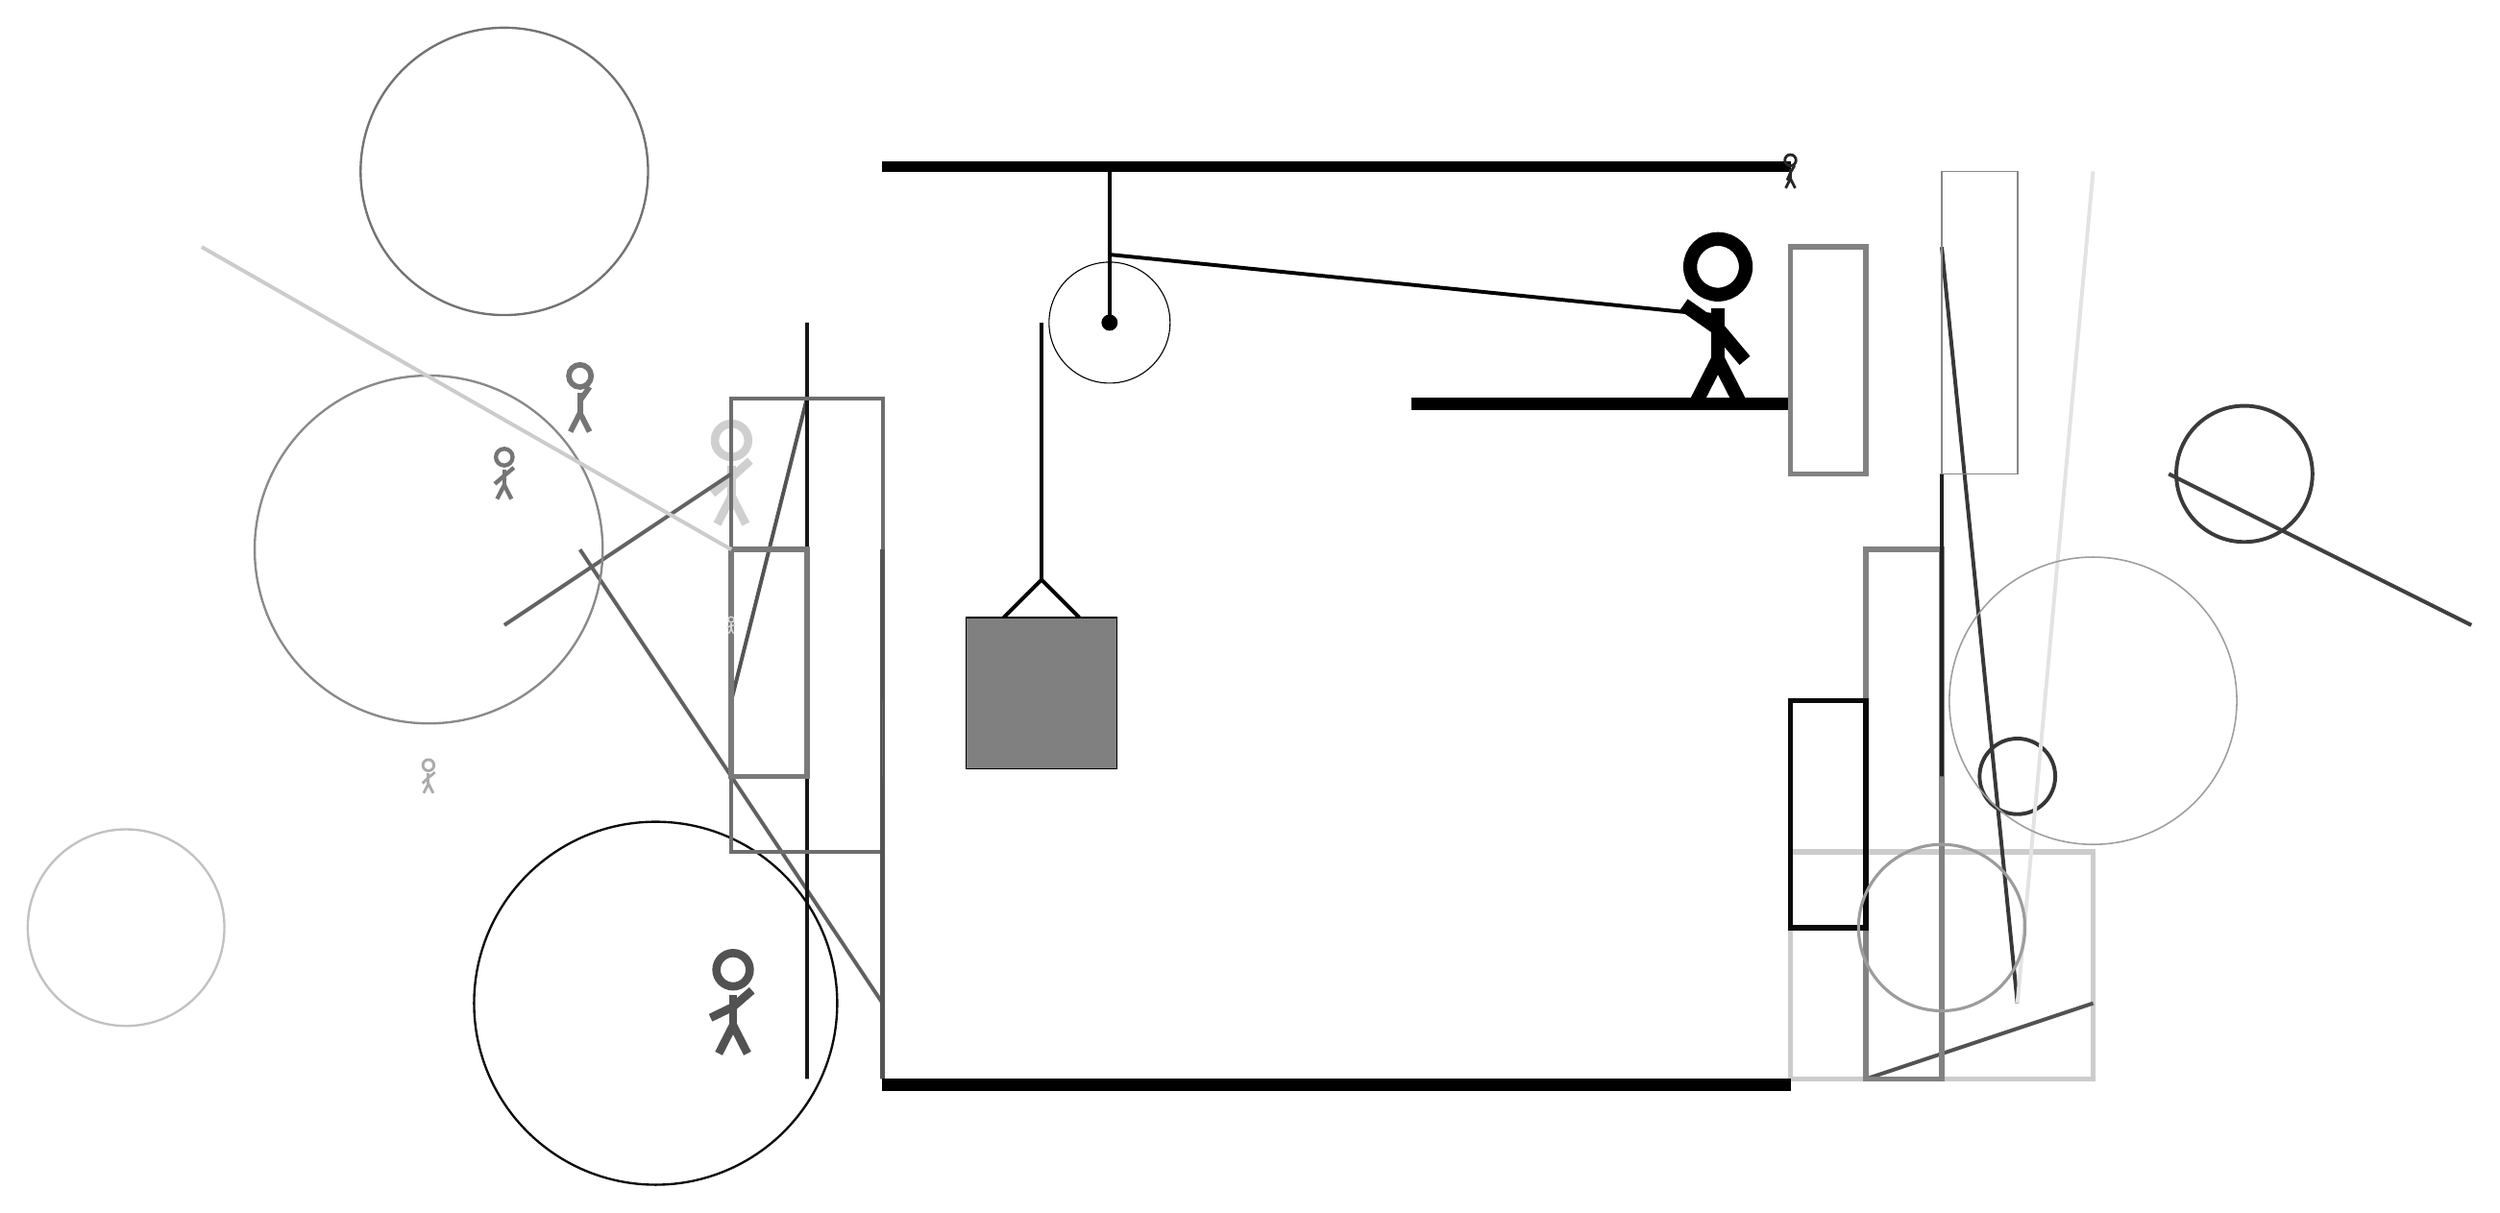
\begin{tikzpicture}
			%%%%% START %%%%%
			
			\draw[fill=black] (-2, 9) rectangle (10, 9.125);
			
			\draw (1, 7) circle (0.8);
			\draw[fill=black] (1, 7) circle (0.1);
			\draw[line width=0.5mm] (1, 9) -- (1, 7);
			
			\draw[line width=0.5mm](-0.4, 3.1) --  (0.1, 3.6) -- (0.6, 3.1);
			\draw[fill=black!50] (-0.9, 3.1) rectangle (1.1, 1.1);
			
			\draw[line width=0.5mm](0.1, 7) -- (0.1, 3.6);
			\centerarc[line width=0.5mm](1, 7)(90:180:0.9)
			\draw[line width=0.5mm](1, 7.9) -- (9, 7.1);
			
			\node at (9, 7) {\Strichmaxerl[10][-35][-50]};
			\draw[fill=black] (5, 6) rectangle (10, 5.85);
			
			\draw[line width=0.7mm, color=black!20] (10, -3) rectangle (14, 0);
			
			\draw [line width=0.5mm, color=black!79](13, 1) circle (0.5);
			\draw [line width=0.3mm, color=black!24](-12, -1) circle (1.3);
			\draw[line width=0.5mm, color=black!75](15, 5) -- (19, 3);
			
			\draw[line width=0.5mm, color=black!78](13, -2) -- (12, 8);
			
			\draw[line width=0.5mm, color=black!68](11, -3) -- (14, -2);
			
			\node[line width=0.6mm, color=black!85] at (10, 9) {\Strichmaxerl[2][67][60]};
			
			\node[line width=0.3mm, color=black!54] at (-6, 6) {\Strichmaxerl[4][90][55]};
			\node[line width=0.2mm, color=black!33] at (-8, 1) {\Strichmaxerl[2][44][39]};
			
			\draw[line width=0.7mm, color=black!49] (11, 4) rectangle (12, -3);
			\node[line width=0.4mm, color=black!19] at (-4, 5) {\Strichmaxerl[6][40][42]};
			\draw[line width=0.5mm, color=black!62](-6, 4) -- (-2, -2);
			\draw[line width=0.4mm, color=black!87] (12, 5) rectangle (12, 1);
			
			\draw [line width=0.5mm, color=black!77](16, 5) circle (0.9);
			\node[line width=0.2mm, color=black!68] at (-4, -2) {\Strichmaxerl[6][26][41]};
			\draw[line width=0.5mm, color=black!67](-4, 2) -- (-3, 6);
			
			\draw[line width=0.5mm, color=black!11](14, 9) -- (13, -2);
			
			\draw[line width=0.5mm, color=black!91] (-3, 7) rectangle (-3, -3);
			\draw [line width=0.3mm, color=black!95](-5, -2) circle (2.4);
			\draw[line width=0.5mm, color=black!57] (-4, 0) rectangle (-2, 6);
			\node[line width=0.6mm, color=black!54] at (-7, 5) {\Strichmaxerl[3][41][40]};
			
			\draw[line width=0.7mm, color=black!96] (11, -1) rectangle (10, 2);
			\draw [line width=0.2mm, color=black!38](14, 2) circle (1.9);
			\draw[line width=0.5mm, color=black!61](-4, 5) -- (-7, 3);
			\draw[line width=0.7mm, color=black!67] (-2, 4) rectangle (-2, -3);
			\draw[line width=0.7mm, color=black!52] (-3, 4) rectangle (-4, 1);
			\draw[line width=0.2mm, color=black!59] (-2, 1) rectangle (-2, 2);
			\draw [line width=0.3mm, color=black!46](-8, 4) circle (2.3);
			\node[line width=0.4mm, color=black!16] at (-4, 3) {\Strichmaxerl[1][22][9]};
			\draw[line width=0.5mm, color=black!20](-4, 4) -- (-11, 8);
			\draw [line width=0.3mm, color=black!55](-7, 9) circle (1.9);
			
			\draw [line width=0.4mm, color=black!39](12, -1) circle (1.1);
			\draw[line width=0.2mm, color=black!47] (12, 5) rectangle (13, 9);
			
			\draw[line width=0.7mm, color=black!49] (11, 8) rectangle (10, 5);
			
			
			\draw[fill=black] (-2, -3) rectangle (10, -3.15);
			
			%%%%% END %%%%%
		\end{tikzpicture}
	\end{figure}	
\end{document}